% ==============================================================================
\section{Módulos de interacción: voz, PLN y salida}
\label{sec:dev_interaccion}
% ==============================================================================

\subsection{Descripción}

Los módulos de interacción son la única interfaz entre el usuario y el sistema. El
usuario habla, el sistema transcribe lo que dijo, interpreta la intención y responde
en voz alta; ninguna función requiere ver una pantalla ni tocar un botón, salvo el
botón opcional para apagar las alertas. Estos módulos atienden RF-01 a RF-06 y los
requerimientos no funcionales RNF-02, RNF-07, RNF-10 y RNF-11.

El reconocimiento de voz, el procesamiento de lenguaje natural (PLN), la personalidad
del asistente y la síntesis de voz los desarrolló el equipo en la carpeta
\texttt{VozYPLN/}. El trabajo de integración consistió en conectar esas piezas con el
navegador y con las alertas en \texttt{interaccion.py}. La Tabla~\ref{tab:inter_partes}
resume los componentes.

\begin{table}[H]
\centering
\caption{Componentes de los módulos de interacción}
\label{tab:inter_partes}
\renewcommand{\arraystretch}{1.25}
\begin{tabular}{|p{3.6cm}|p{10.9cm}|}
\hline
\textbf{Componente} & \textbf{Función} \\
\hline
\texttt{voz\_recog.py} & Reconocimiento de voz sin conexión con Vosk (modelo
\texttt{vosk-model-small-es-0.42}) a 16~kHz. \\
\hline
\texttt{PLN\_oneimport.py} & Clasificación de la intención y extracción del destino. \\
\hline
\texttt{dialogo.py} & Frases con la personalidad del asistente (``Guía''). \\
\hline
\texttt{Tts.py} & Síntesis de voz con edge-tts (voz \texttt{es-MX-DaliaNeural}) y respaldo
local con pyttsx3. \\
\hline
\texttt{interaccion.py} & Integración: cola de voz con prioridades, escucha en segundo
plano y traducción de intenciones a comandos del navegador. \\
\hline
\end{tabular}
\end{table}

Respecto al diseño de TT1 hubo tres cambios. El detector de actividad de voz y el
filtro de Wiener que se habían planteado como etapas previas no se implementaron por
separado: Vosk detecta por sí mismo el final de cada frase y el filtro no mejoró el
reconocimiento en las primeras pruebas. El PLN no usa spaCy, sino un clasificador
propio escrito en Python puro, que combina reglas con una red neuronal pequeña. Y la
síntesis de voz usa una voz neuronal en línea con un respaldo local, en lugar de
depender solo de pyttsx3.

\subsection{Reconocimiento de voz}

El reconocedor captura audio del micrófono en bloques de 0.25~s y los entrega a Vosk.
Cuando Vosk detecta que la frase terminó, devuelve el texto y el reconocedor lo coloca
en una cola que el ciclo principal revisa en cada cuadro. La escucha corre en un hilo
aparte, de modo que el sistema sigue percibiendo y navegando mientras espera una
orden. Mientras el sistema habla, lo que capta el micrófono se descarta, porque lo más
probable es que se esté escuchando a sí mismo. Si no hay micrófono o falta el modelo de
Vosk, el sistema lo avisa y acepta las órdenes por teclado, lo cual se usa durante el
desarrollo.

\subsection{Procesamiento de lenguaje natural}

El PLN recibe el texto transcrito y devuelve una de 14 intenciones, el destino si lo
hay, un valor de confianza y una respuesta sugerida. Las intenciones son: destino,
pausa, reanudar, detener, ruta alternativa, emergencia, ubicación, entorno, repetir,
cancelar, ayuda, confirmar, negar y estado de la ruta. El proceso tiene cuatro pasos:

\begin{enumerate}
    \item \textbf{Normalización.} El texto se pasa a minúsculas, se quitan los acentos
    y los signos, y se divide en palabras. Se descartan palabras sin contenido (``el'',
    ``por favor'') y se agregan sinónimos conocidos.
    \item \textbf{Palabras de seguridad.} Si el texto contiene una palabra como
    ``detente'', ``alto'', ``auxilio'' o ``cancela'', la intención se fija de inmediato
    con confianza de 0.99, sin consultar a los clasificadores.
    \item \textbf{Clasificación.} Se calculan dos puntuaciones para cada intención. La
    de reglas compara el texto con 121 frases de referencia mediante similitud de
    palabras basada en la distancia de Levenshtein, que tolera errores del
    reconocedor, y similitud de coseno entre bolsas de palabras. La de la red neuronal
    usa una capa oculta de 24 neuronas sobre un vector TF-IDF, entrenada con 164
    ejemplos (las frases de referencia más variantes con sinónimos). Ambas se combinan
    con un peso para la red que crece con el número de ejemplos aprendidos y con la
    proporción de palabras del texto que la red conoce. Si la mejor puntuación es
    menor que 0.42, o si las dos mejores quedan casi empatadas, el resultado es
    ``desconocido'' y el sistema pide repetir.
    \item \textbf{Destino.} Para la intención de destino se busca primero un lugar
    conocido por similitud, después lo que sigue a frases como ``llévame a'' o
    ``quiero ir a'' y, como último recurso, las palabras que quedan al quitar las de
    navegación. Si no hay destino, el sistema pregunta ``¿A dónde te gustaría ir?'' y
    toma la siguiente frase como respuesta.
\end{enumerate}

El PLN puede aprender frases nuevas cuando recibe una corrección, y las guarda en un
archivo local. Para la evaluación de esta sección se usó el modelo sin frases
aprendidas, que es el que tendría un usuario nuevo.

\subsection{Integración con el navegador}

La clase \texttt{Interaccion} convierte cada intención en una acción. Las de la
sesión (destino, pausa, reanudar, detener, cancelar, ruta alternativa, ubicación y
estado) se envían al navegador como comandos. El destino se limpia antes de enviarlo
(se quitan artículos y plurales, porque el PLN puede devolver ``la puerta'' o
``baños'') y se traduce a la etiqueta del \emph{landmark} con un diccionario de
sinónimos: ``salida'', ``puerta'' y ``entrada'' se buscan como \emph{door}; ``baño''
como \emph{toilet}; ``escritorio'' como \emph{desk}, y así para 38 palabras. Las demás
intenciones se resuelven en la misma clase:

\begin{itemize}
    \item \textbf{Entorno} (``¿qué hay enfrente?''): describe el objeto más cercano en
    cada sector, o la distancia libre si no hay ninguno. La frase tiene la forma ``Al
    frente, door a 2 metros. A la izquierda libre. A la derecha, chair a 90
    centímetros'': el nombre del objeto se dice con la etiqueta en inglés del
    detector, lo cual es una deficiencia pendiente.
    \item \textbf{Repetir}: vuelve a decir la última indicación de navegación.
    \item \textbf{Emergencia}: emite un aviso con prioridad máxima y pausa la
    navegación. El aviso a un contacto de emergencia quedó pendiente.
    \item \textbf{Ayuda}: enumera lo que se puede decir.
\end{itemize}

Las frases ``apagar sistema'' y ``terminar programa'' cierran el sistema con una
despedida.

\subsection{Salida de voz}

Todo lo que el sistema dice pasa por una cola con tres prioridades: 0 para alertas, 1
para indicaciones de navegación y 2 para respuestas y confirmaciones. Un mensaje de
prioridad 0 interrumpe lo que se esté diciendo. Las indicaciones de navegación forman
un canal especial en el que solo se dice la más reciente: si el sintetizador va
atrasado y en la cola hay un ``gire a la izquierda'' viejo, se descarta, porque ya no
corresponde a la posición del usuario; también se descartan las indicaciones que
llevan más de 6~s esperando. Mientras suena un pitido de alerta, la cola espera.

La síntesis usa edge-tts con la voz neuronal \texttt{es-MX-DaliaNeural}, que suena
natural pero necesita conexión a internet. Cada frase sintetizada se guarda en un
archivo, así que las frases repetidas (que son la mayoría) se reproducen sin conexión.
Si la conexión falla, el sistema cambia a pyttsx3, que usa la voz instalada en el
sistema operativo; si tampoco está disponible, escribe las frases en consola.

\subsection{Personalidad del asistente}

El navegador genera las frases literales definidas en TT1 (``Avance 3 metros'',
``Gire ligeramente a la izquierda''). Con el modo amigable activado, que es el
predeterminado, \texttt{dialogo.py} las reformula con un tono más cercano: la
distancia se expresa en pasos, los giros con referencias cotidianas y las frases
varían para no sonar repetitivas (Tabla~\ref{tab:inter_frases}). La frase
``Deténgase'' y las alertas no se reformulan, porque en esos casos importa más la
rapidez que la amabilidad.

\begin{table}[H]
\centering
\caption{Frases literales del navegador y su versión amigable}
\label{tab:inter_frases}
\renewcommand{\arraystretch}{1.25}
\begin{tabular}{|p{5.2cm}|p{9.3cm}|}
\hline
\textbf{Literal (TT1)} & \textbf{Amigable (dialogo.py)} \\
\hline
Ruta calculada. Iniciando navegación. & Muy bien, te llevo a sillon. Vamos paso a
paso. \\
\hline
Gire ligeramente a la izquierda & Perfecto, da una vuelta suave a tu izquierda. \\
\hline
Gire a la derecha 90 grados & Listo, da vuelta completa a tu derecha, como una
esquina. \\
\hline
Avance 3 metros & Vas muy bien, continúa de frente unos 4 pasos. \\
\hline
Ha llegado a su destino. & ¡Listo, llegamos a door! \\
\hline
Deténgase & Deténgase (sin cambio) \\
\hline
\end{tabular}
\end{table}

Una sutileza de la integración: \texttt{dialogo.py} considera positivos los giros a la
derecha, mientras que en el resto del sistema los ángulos positivos son hacia la
izquierda. La conversión invierte el signo; las pruebas automatizadas verifican que
un giro a la izquierda del navegador se diga ``a tu izquierda''.

El Algoritmo~\ref{alg:dev_inter} resume el manejo de una frase del usuario.

\begin{center}
\captionof{algorithm}{Manejo de una frase del usuario}
\label{alg:dev_inter}
\end{center}
\vspace{-1.8cm}
\rule{\textwidth}{0.4pt}
\vspace{-0.9cm}
\begin{algorithmic}[1]

\Statex \textbf{ENTRADA:} texto (de Vosk o del teclado), cuadro\_nav
\Statex \textbf{SALIDA:} mensajes para la cola de voz

\Statex
\If{texto es ``apagar sistema'' o ``terminar programa''}
    \State \Return [despedida]
\EndIf
\If{se esperaba la respuesta a ``¿a dónde te gustaría ir?''}
    \State texto $\gets$ ``llévame a '' + texto
\EndIf
\State r $\gets$ PLN.procesar(texto)
\If{r.intención = destino}
    \If{no hay destino}
        \State marcar que se espera respuesta
        \State \Return [``¿A dónde te gustaría ir?'']
    \EndIf
    \State etiqueta $\gets$ sinónimos(limpiar(r.destino))
    \State msgs $\gets$ navegador.comando(navegar, etiqueta, cuadro\_nav)
\ElsIf{r.intención es de sesión}
    \State msgs $\gets$ navegador.comando(r.intención)
\ElsIf{r.intención = entorno}
    \State msgs $\gets$ [describir\_entorno(cuadro\_nav)]
\ElsIf{r.intención = emergencia}
    \State msgs $\gets$ [aviso con prioridad 0] + navegador.comando(pausa)
\Else
    \State msgs $\gets$ [respuesta según la intención]
\EndIf
\If{modo amigable}
    \State reformular las confirmaciones con dialogo.py
\EndIf
\State \Return msgs

\end{algorithmic}
\vspace{-0.9cm}
\rule{\textwidth}{0.4pt}

\subsection{Resultados}

\textbf{Evaluación del PLN.} Para medir el PLN con frases que no conociera, se
redactó un conjunto de 102 frases de prueba, distintas de las frases de referencia,
con la intención correcta de cada una (por ejemplo, ``espérame tantito'' para pausa o
``ya no quiero seguir'' para detener). El conjunto se escribió antes de correr la
evaluación y no se modificó después de ver los resultados. El PLN acertó la intención
en 80 de las 102 frases (78.4\,\%). En las frases de destino, extrajo correctamente
el lugar en 16 de 21. Procesar una frase tomó en promedio 2.8~ms (máximo 7~ms). La
Figura~\ref{fig:pln_confusion} muestra la matriz de confusión.

\begin{figure}[H]
    \centering
    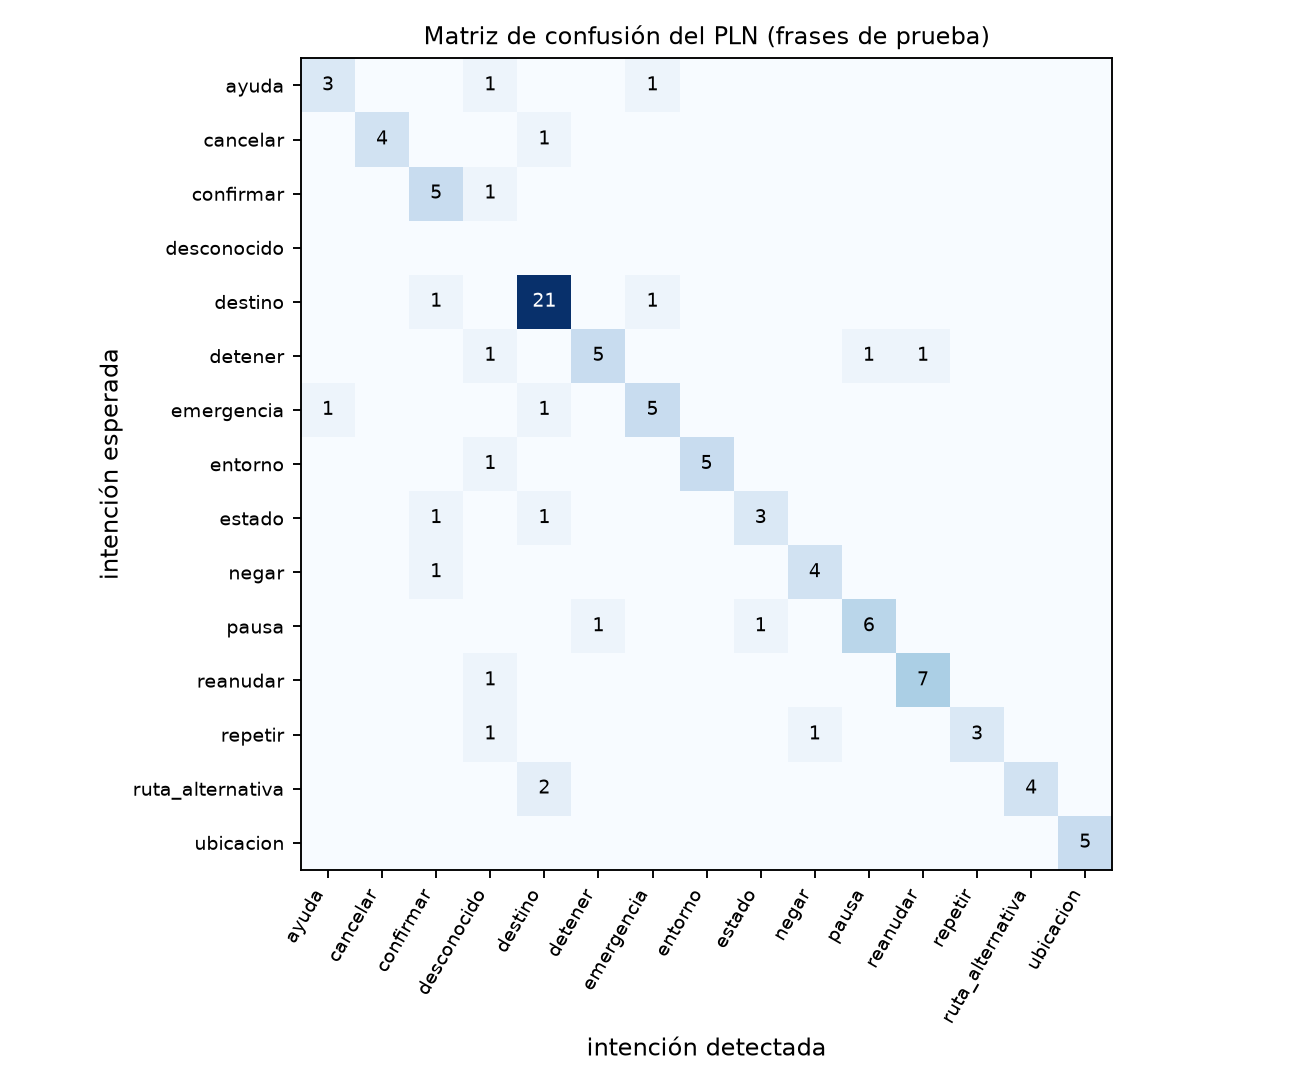
\includegraphics[width=0.78\textwidth]{Capturas_TT2/voz/pln_confusion.png}
    \caption{Matriz de confusión del PLN sobre las 102 frases de prueba.}
    \label{fig:pln_confusion}
\end{figure}

La mayoría de los errores son inofensivos: la frase cae en ``desconocido'' y el
sistema pide repetir, o el destino se extrae con palabras de sobra (``llevas banca'',
``guiar mesa''), lo que hace que no se encuentre el lugar. Algunos, sin embargo, son
delicados por su efecto sobre la navegación:

\begin{itemize}
    \item ``ya no quiero seguir'' se interpretó como reanudar, y ``termina la
    navegación'' como pausa;
    \item ``no es correcto'' se interpretó como confirmar;
    \item ``ayuda'' se interpretó como emergencia y, al revés, ``ayuda, me caí'' como
    una petición de ayuda sobre los comandos;
    \item ``detente un momento por favor'' se interpretó como detener en lugar de
    pausa, por la palabra de seguridad ``detente''. Esta última es una decisión de
    diseño conservadora y se considera aceptable.
\end{itemize}

\textbf{Reconocimiento de voz con ruido.} Para evaluar la cadena completa sin
voluntarios se generó audio con las 10 voces en español disponibles en macOS (dos
voces naturales, Paulina y Mónica, y ocho voces de estilo caricaturesco) diciendo 30
comandos de uso frecuente. Cada audio se pasó por Vosk y por el PLN en limpio y
mezclado con ruido rosa a 20, 10 y 5~dB de relación señal a ruido. Un comando cuenta
como correcto si produce la acción esperada y, en los de destino, el lugar correcto.
Los resultados se muestran en la Tabla~\ref{tab:asr} y en la
Figura~\ref{fig:asr_ruido}.

\begin{table}[H]
\centering
\caption{Voz sintetizada, Vosk y PLN (300 audios por condición)}
\label{tab:asr}
\renewcommand{\arraystretch}{1.2}
\begin{tabular}{|l|c|c|c|}
\hline
\textbf{Condición} & \textbf{WER} & \textbf{Comandos correctos} &
\textbf{Correctos, voces naturales} \\
\hline
Limpio & 22.2\,\% & 80.0\,\% & 91.7\,\% \\
20~dB & 23.8\,\% & 78.3\,\% & 81.7\,\% \\
10~dB & 33.0\,\% & 71.0\,\% & 63.3\,\% \\
5~dB & 43.1\,\% & 58.7\,\% & 45.0\,\% \\
\hline
\end{tabular}
\end{table}

\begin{figure}[H]
    \centering
    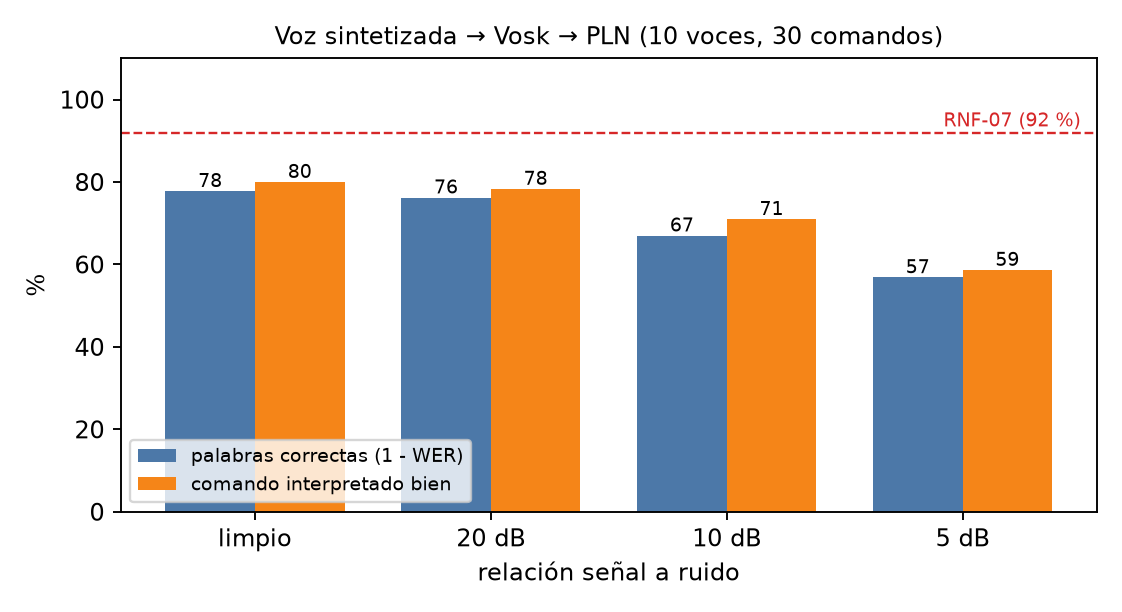
\includegraphics[width=0.75\textwidth]{Capturas_TT2/voz/asr_ruido.png}
    \caption{Palabras correctas y comandos bien interpretados según el nivel de ruido.}
    \label{fig:asr_ruido}
\end{figure}

En audio limpio con las voces naturales el sistema interpreta bien el 91.7\,\% de los
comandos, prácticamente en el 92\,\% que pide RNF-07. Con ruido el desempeño cae
rápido. Una voz hablada a corta distancia del micrófono en un entorno de 60~dB
(el nivel que menciona RNF-07) equivale aproximadamente a la franja de 5 a 10~dB de la
tabla, donde los comandos correctos están entre 59 y 71\,\%. Por lo tanto, el
requerimiento no se cumple en condiciones ruidosas. También se observó que, en los
194 audios limpios que Vosk transcribió sin ningún error, el PLN acertó en 181
(93\,\%); el resto del error en limpio proviene del reconocimiento.

En cuanto a la latencia, una vez que termina el audio Vosk entrega el resultado final
en 8~ms en promedio (17~ms en el percentil 95) y el PLN tarda 2~ms. Esta medición no
incluye el tiempo que Vosk espera en silencio para decidir que la frase terminó,
que en uso real se suma a la latencia percibida. Aun así, el procesamiento queda muy
por debajo de los 500~ms de RNF-02.

Las pruebas automatizadas de la interacción (24) verifican la traducción de
intenciones a comandos, la aclaración de destino en dos turnos, la limpieza de
destinos, la conversión de signo de los giros, la descripción del entorno y el
funcionamiento sin micrófono ni sintetizador.

\subsection{Limitaciones}

\begin{itemize}
    \item El PLN acierta el 78\,\% de las frases nuevas y comete errores que invierten el
    sentido de la orden (detener interpretado como reanudar). Ampliar las frases de
    referencia con las formas que usan las personas y revisar las palabras de seguridad
    son los pasos inmediatos.
    \item Con ruido de calle, el reconocimiento queda lejos del 92\,\% de RNF-07.
    \item La evaluación de voz usó voces sintéticas; falta probar con personas reales,
    con distintos acentos y con el micrófono del prototipo.
    \item La voz neuronal requiere internet la primera vez que se dice cada frase; sin
    conexión se usa una voz del sistema mucho menos natural.
    \item La llegada y la descripción del entorno mencionan las etiquetas en inglés
    del detector (``llegamos a door'', ``chair a 90 centímetros''). Hace falta un
    diccionario inverso de etiquetas a nombres en español.
    \item El aviso a un contacto de emergencia no está implementado.
\end{itemize}
